
%(BEGIN_QUESTION)
% Copyright 2008, Tony R. Kuphaldt, released under the Creative Commons Attribution License (v 1.0)
% This means you may do almost anything with this work of mine, so long as you give me proper credit

Determine both the input and output voltage in this circuit:

$$\includegraphics[width=15.5cm]{i03262x01.eps}$$

\vskip 20pt \vbox{\hrule \hbox{\strut \vrule{} {\bf Suggestions for Socratic discussion} \vrule} \hrule}

\begin{itemize}
\item{} When analyzing opamp circuits, it is helpful to bear in mind the ``simplifying assumptions'' of negative-feedback opamp circuits.  Identify some of these assumptions, especially the one regarding input voltages to the opamp when negative feedback is in effect.
\item{} Identify which fundamental principles of electric circuits apply to each step of your analysis of this circuit.  In other words, be prepared to explain the reason(s) ``why'' for every step of your analysis, rather than merely describing those steps.
\item{} Identify all the effects of the 18 k$\Omega$ resistor failing open.
\item{} Identify all the effects of the 5 k$\Omega$ resistor failing open.
\item{} Identify all the effects of the 18 k$\Omega$ resistor failing shorted.
\item{} Identify all the effects of the 5 k$\Omega$ resistor failing shorted.
\end{itemize}

\underbar{file i03262}
%(END_QUESTION)





%(BEGIN_ANSWER)

$V_{in}$ = 10 V \hskip 30pt $V_{out}$ = 46 V

%(END_ANSWER)





%(BEGIN_NOTES)

Ask your students how they solved this problem, sharing techniques and strategies to help other students know where to begin and where to proceed from there.  They should be able to label all voltage polarities and all current directions.

%INDEX% Electronics review: opamp noninverting amplifier circuit

%(END_NOTES)


